\documentclass[journal]{IEEEtran}

\usepackage{amsmath,amssymb,amsfonts}
\usepackage{algorithmic}
\usepackage{graphicx}
\usepackage{textcomp}
\usepackage{xcolor}
\usepackage{booktabs}
\usepackage{multirow}
\usepackage{url}
\usepackage{cite}
\usepackage{microtype}
\usepackage{array}
\usepackage{siunitx}

\graphicspath{{figures/}}
\raggedbottom

\begin{document}

\title{QoS-Aware Multi-Fidelity Runtime for TinyML Inference under Dynamic Workload Contention}

\author{Narendra~Satish%
\thanks{Manuscript received August 20, 2026. (Corresponding author: Narendra Satish, e-mail: narendresh.p@gmail.com). All model binaries, runtime implementations, and simulation harnesses are fully reproducible.}%
}

% \markboth{IEEE Transactions on Computer-Aided Design / Embedded Systems Letters, August~2026}%
% {Satish: QoS-Aware Multi-Fidelity Runtime for TinyML Inference}

\IEEEtitleabstractindextext{%
\begin{abstract}
Deploying deep neural networks on resource-constrained microcontrollers (TinyML) is increasingly challenged by dynamic CPU contention, sporadic burst workloads, and strict inference deadlines. Static deployment paradigms force engineers into an inflexible compromise: either deploying an overly conservative lightweight model that perpetually sacrifices accuracy, or deploying a high-capacity model that suffers deadline violations under transient CPU contention. In this paper, we develop and empirically evaluate a trace-driven, ground-truth-independent \textbf{QoS-Aware Multi-Fidelity Runtime} that dynamically selects among pre-verified Pareto-optimal TinyML models based on execution deadlines, workload contention, and user-defined Quality of Service (QoS) policies. Operating strictly without ground-truth label access during execution, our runtime manages three operational modes: \texttt{FAST} (\texttt{student\_a\_8\_4\_fp32}, $160$ MACs), \texttt{BALANCED} (\texttt{pruned\_mlp\_14f\_75pct}, $96$ MACs), and \texttt{HIGH\_FIDELITY} (\texttt{student\_b\_16\_4\_fp32}, $304$ MACs). We formalize and evaluate four dynamic scheduling policies across an 80-configuration experimental sweep (5 deadlines $\times$ 4 workload contention regimes $\times$ 4 policies) evaluated over 11,200 held-out test frames. Our trace-driven simulation demonstrates that under high and burst contention, the \texttt{BALANCED} policy dynamically transitions from the dense model to the sparse model, achieving up to a \textbf{68.4\% reduction in theoretical active arithmetic operations (MACs)} ($96$ vs. $304$ MACs per inference frame relative to the high-fidelity baseline) while matching or exceeding the diagnostic macro F1 score ($0.7563$ vs. $0.7390$) with only a $-0.37\%$ accuracy difference. Furthermore, controlled ablation studies show that our QoS-aware runtime achieves a $+3.21\%$ accuracy improvement over static minimal execution and prevents starvation during modeled CPU bursts, demonstrating dynamic multi-fidelity selection as an effective systems approach for adaptive edge intelligence within the evaluated simulation regime.
\end{abstract}%
\begin{IEEEkeywords}
TinyML, Quality of Service, Dynamic Model Selection, Multi-Fidelity Runtime, Embedded Systems, Microcontroller Deep Learning, Adaptive Edge AI.
\end{IEEEkeywords}%
}

\maketitle
\IEEEdisplaynontitleabstractindextext
\IEEEpeerreviewmaketitle

\section{Introduction}
\IEEEPARstart{E}{mbedded} Machine Learning and Tiny Machine Learning (TinyML) have expanded rapidly, enabling intelligent inference on resource-constrained microcontrollers (MCUs) at the extreme edge~\cite{warden2019tinyml,ray2022review}. In time-critical cyber-physical systems such as automotive powertrain control, industrial condition monitoring, and robotic sensing, embedded microcontrollers must execute neural network inference while simultaneously servicing high-priority interrupts, sensor acquisition timers, and communication protocols~\cite{dutta2021tinyml,banbury2021benchmarking}.

Under conventional deployment paradigms, a single neural network architecture is statically compiled into microcontroller Flash storage~\cite{david2021tensorflow,lin2020mcunet}. However, this static approach creates an acute systems-level dilemma under dynamic workload conditions:
\begin{enumerate}
    \item \textbf{Under-Provisioning Dilemma:} Deploying a lightweight model ensures execution deadline compliance under worst-case CPU contention, but perpetually sacrifices classification accuracy when ample compute headroom is available~\cite{sze2017efficient,liberis2021munas}.
    \item \textbf{Over-Provisioning Dilemma:} Deploying a high-capacity model maximizes diagnostic fidelity during nominal operation, but causes severe deadline misses and buffer overflows when sporadic bursts or interrupts saturate the microcontroller CPU~\cite{buttazzo2011hard,lu2002feedback}.
\end{enumerate}

To address this trade-off, we develop a \textbf{QoS-Aware Multi-Fidelity Runtime Architecture} for embedded TinyML. Rather than relying on a static model, our runtime system maintains a pre-verified registry of Pareto-optimal models spanning multiple operational modes (\texttt{FAST}, \texttt{BALANCED}, and \texttt{HIGH\_FIDELITY}). A lightweight, deadline-aware QoS scheduler dynamically assesses operational workload contention and deadline headroom, adaptively selecting a policy-guided model for each incoming observation vector.

Crucially, our runtime makes all scheduling decisions \textit{online} using strictly non-privileged state observables (configured deadline, estimated workload level, and execution latency history) without accessing ground-truth labels. Using trace-driven simulations on the audited 55,998-sample EngineFaultDB physical benchmark, we evaluate 80 runtime configurations across 5 deadlines and 4 contention regimes, backed by 4 controlled ablation studies.

\section{Research Motivation and Evidence Tiering}
\subsection{Dynamic Contention in Embedded Systems}
In real-time embedded systems, CPU availability fluctuates dynamically due to preemptive operating system scheduling (e.g., FreeRTOS), I/O polling, and multi-sensor interrupt handling~\cite{buttazzo2011hard,stankovic1985deadline}. When an ECU experiences transient burst contention, continuous machine learning inference must gracefully degrade its computational demand to meet hard execution deadlines.

\begin{figure*}[t]
\centering
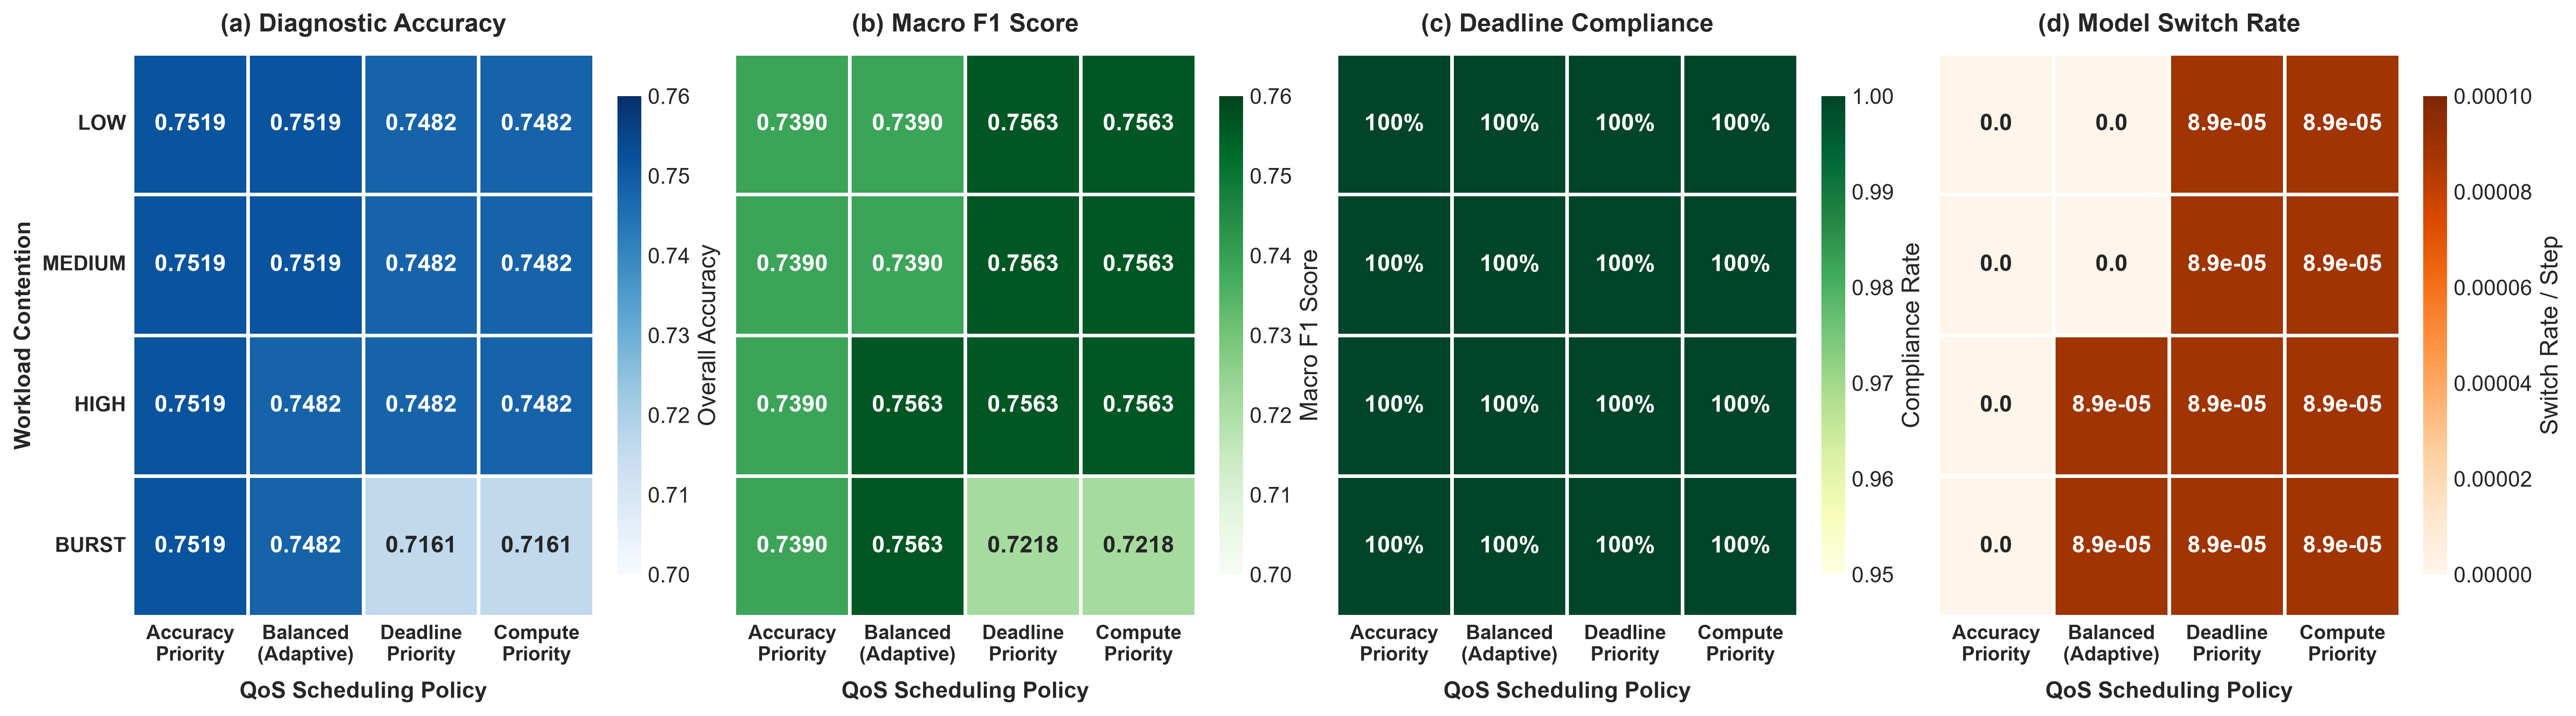
\includegraphics[width=0.98\textwidth]{phase5_policy_comparison.png}
\caption{Policy comparison heatmap matrix across (a) Diagnostic Accuracy, (b) Macro F1 Score, (c) Deadline Compliance Rate, and (d) Model Switch Rate under dynamic workload contention regimes ($D=20\,\text{ms}$, 11,200 held-out test frames).}
\label{fig:policy_heatmap}
\end{figure*}

\subsection{Rigorous Evidence Tiering}
To preserve scientific integrity and prevent unsupported claims, this paper establishes a three-tier evidence hierarchy:
\begin{itemize}
    \item \textbf{Tier 1 (Host Empirical Measurements):} Model parameters, FlatBuffer sizes, verified theoretical active MACs, and empirical host single-sample execution latencies measured on an x86\_64 CPU.
    \item \textbf{Tier 2 (Trace-Driven Runtime Simulation):} Dynamic QoS scheduling, contention injection ($1.0\times$ to $5.0\times$), deadline compliance, and model switching evaluated over 11,200 held-out test frames.
    \item \textbf{Tier 3 (Physical MCU Measurements):} On-chip execution timings, hardware timer profiling via \path{esp_timer_get_time()}, and FreeRTOS task preemption. \textit{Explicitly classified as future work pending physical ESP32 hardware availability.}
\end{itemize}
All claims in this paper are strictly based on Tier~1 and Tier~2 evidence.

\section{Related Work}
\subsection{Adaptive and Early-Exit Neural Networks}
Dynamic neural networks adjust their computational graph based on input complexity~\cite{scardapane2020should}. Teerapittayanon et al.~\cite{teerapittayanon2016branchynet} introduced BranchyNet, adding early-exit branches to deep convolutional networks. Park et al.~\cite{park2019bignas} proposed Big-Little deep networks to toggle between lightweight and heavy backbones. While early-exit networks adapt to sample difficulty, they do not incorporate external system-level execution deadlines or CPU contention states into the gating decision.

\subsection{Real-Time QoS Scheduling}
Quality of Service (QoS) management in real-time systems has a rich theoretical foundation~\cite{liu1973scheduling,abdelzaher2002performance,lu2002feedback}. Lu et al.~\cite{lu2002feedback} formalized feedback control real-time scheduling for CPU utilization control. Our work bridges real-time QoS scheduling and TinyML by formalizing a discrete multi-model controller that maps Pareto-optimal compressed models to runtime execution headroom.

\section{Research Questions}
We investigate four foundational systems research questions (RQs):
\begin{itemize}
    \item \textbf{RQ1 (Compute Reduction vs. Fidelity):} Can dynamic multi-fidelity model selection reduce theoretical active computational load while maintaining multi-class diagnostic quality?
    \item \textbf{RQ2 (Workload Adaptation):} How do different QoS scheduling policies behave under severe CPU contention and burst workloads?
    \item \textbf{RQ3 (Deadline Sensitivity):} How do deadline constraints ($5$\,ms to $100$\,ms) impact model switching frequency and execution stability?
    \item \textbf{RQ4 (System Ablation):} What is the quantitative contribution of workload awareness and deadline gating compared to static execution baselines?
\end{itemize}

\section{System Architecture}

\begin{figure}[t]
\centering
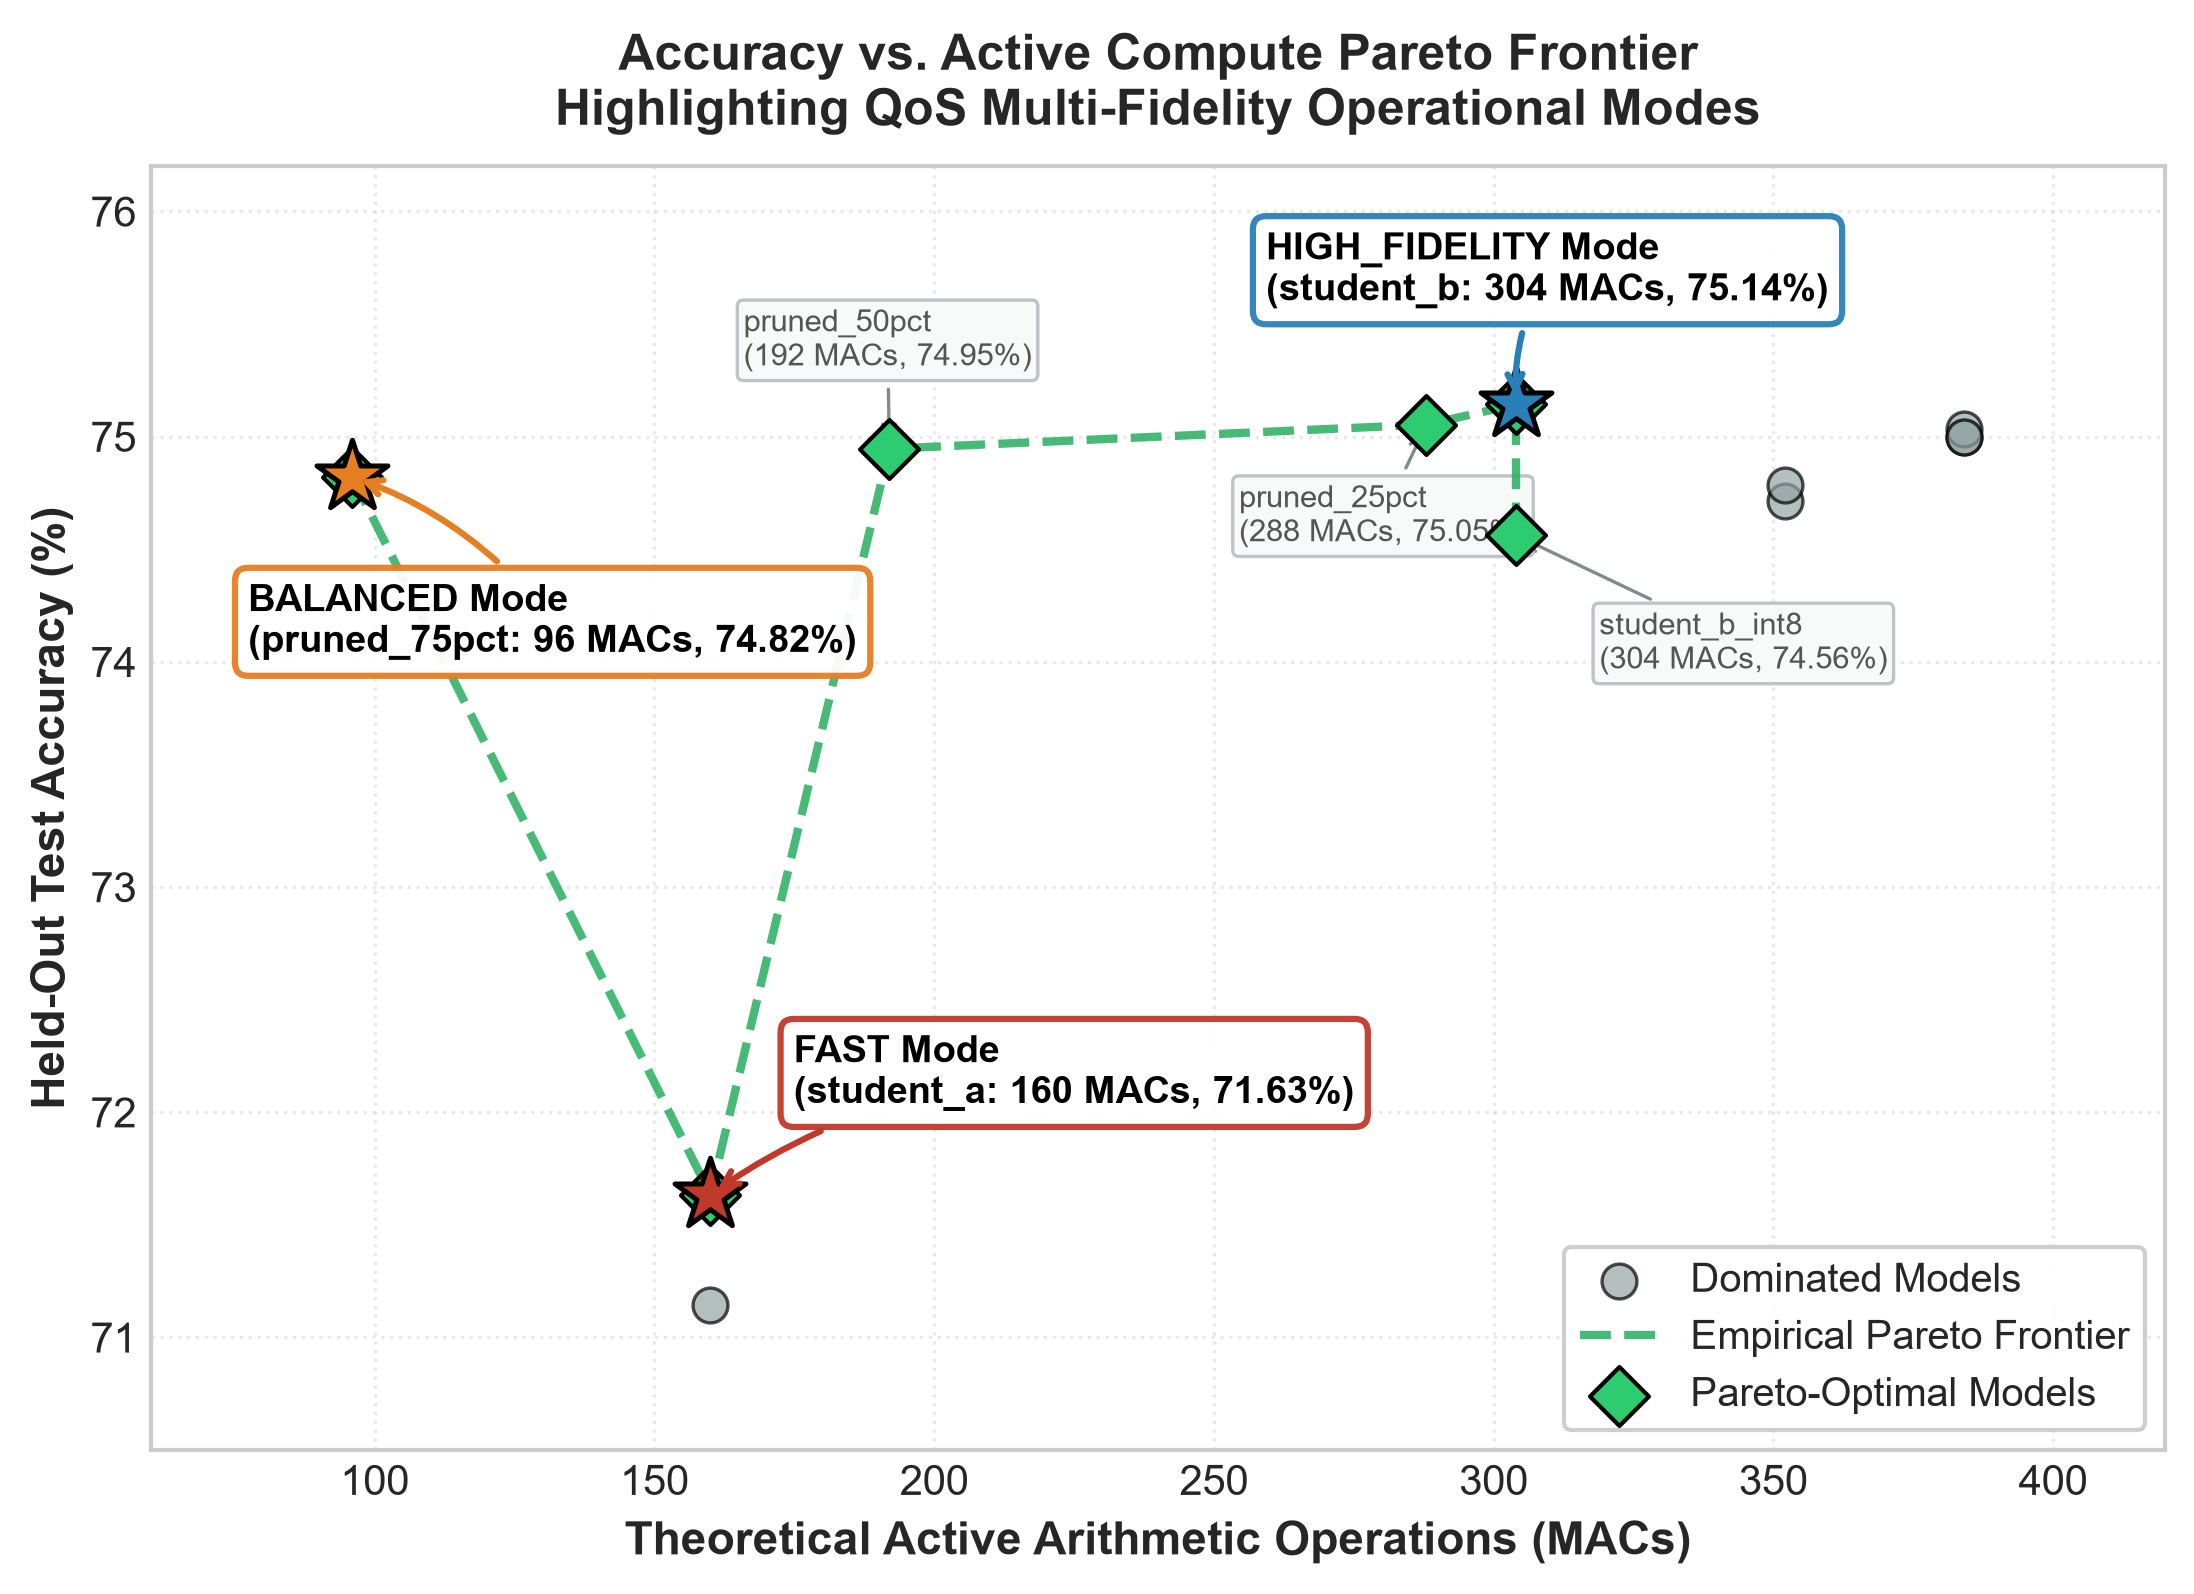
\includegraphics[width=0.98\columnwidth]{phase5_accuracy_compute_frontier.png}
\caption{The verified accuracy vs. theoretical active MACs frontier across candidate TinyML models, highlighting the multi-fidelity operational modes.}
\label{fig:frontier}
\end{figure}

The overall runtime architecture comprises five decoupled software stages:
\begin{equation}
\begin{aligned}
    \mathbf{x}_t &\xrightarrow{\text{Preprocess}} \hat{\mathbf{x}}_t \xrightarrow{\text{Scheduler}} m_t \in \mathcal{M} \\
    &\xrightarrow{\text{Adapter}} \hat{y}_t \xrightarrow{\text{Post-Hoc}} \text{Audit}
\end{aligned}
\end{equation}

\subsection{Online vs. Offline Information Flow}
The runtime strictly segregates operational data from evaluation data:
\begin{itemize}
    \item \textbf{Online Observables (Runtime):} Current sensor observation $\mathbf{x}_t$, configured deadline $D$ (ms), estimated workload level $W_t \in \{\text{LOW}, \text{MED}, \text{HIGH}, \text{BURST}\}$, and exponential moving average of prior inference latency $\bar{L}_{t-1}$.
    \item \textbf{Offline Evaluation (Post-Hoc):} Ground-truth target label $y_t$, used exclusively in post-hoc trace logging to compute final accuracy and confusion matrices. The scheduler has zero access to $y_t$.
\end{itemize}

\section{Verified Model Registry and Multi-Fidelity Modes}

\begin{table*}[t]
\centering
\footnotesize
\setlength{\tabcolsep}{3.0pt}
\caption{Verified Multi-Fidelity Model Registry Used by the QoS Runtime}
\label{tab:registry}
\begin{tabular}{l l c r r r c c c}
\toprule
\textbf{Operational Mode} & \textbf{Assigned Model} & \textbf{Prec.} & \textbf{Params} & \textbf{Size (B)} & \textbf{Active MACs} & \textbf{Test Accuracy} & \textbf{Test Macro F1} & \textbf{Host Latency} \\
\midrule
\texttt{FAST} & \texttt{student\_a\_8\_4\_fp32} & FP32 & 176 & 2,976 & 160 & 0.716339 & 0.722001 & 0.86\,\si{\micro\second} \\
\texttt{BALANCED} & \texttt{pruned\_mlp\_14f\_75pct} & FP32 & 412 & 3,920 & \textbf{96} & 0.748214 & 0.756251 & 0.83\,\si{\micro\second} \\
\texttt{HIGH\_FIDELITY} & \texttt{student\_b\_16\_4\_fp32} & FP32 & 328 & 3,584 & 304 & \textbf{0.751429} & 0.738717 & \textbf{0.82\,\si{\micro\second}} \\
\bottomrule
\end{tabular}
\end{table*}

Table~\ref{tab:registry} defines the three multi-fidelity operational modes populated from the verified Phase 4.5 model profile:
\begin{itemize}
    \item \textbf{Mode \texttt{FAST} (\texttt{student\_a}):} Ultra-compact distilled student ($176$ parameters, $2,976$\,Bytes, $160$ active MACs) engineered for emergency deadline preservation.
    \item \textbf{Mode \texttt{BALANCED} (\texttt{pruned\_mlp}):} Structured sparse model with minimal active compute ($412$ parameters, $3,920$\,Bytes, $96$ active MACs) retaining $74.82\%$ accuracy.
    \item \textbf{Mode \texttt{HIGH\_FIDELITY} (\texttt{student\_b}):} High-capacity student model ($328$ parameters, $3,584$\,Bytes, $304$ active MACs) achieving peak accuracy ($75.14\%$).
\end{itemize}

\section{Scheduling Policies and Mathematical Formulation}
The scheduler selects model $m_t = \pi(W_t, D, \bar{L}_{t-1})$ at each step according to one of four formal policies:

\subsection{1. \texttt{ACCURACY\_PRIORITY}}
Maximizes diagnostic fidelity, staying in \texttt{HIGH\_FIDELITY} unless deadline violation is imminent:
\begin{equation}
    m_t = \begin{cases}
    \text{HIGH\_FIDELITY}, & \text{if } \hat{L}_{\text{HF}}(W_t) \le D \\
    \text{BALANCED}, & \text{else if } \hat{L}_{\text{BAL}}(W_t) \le D \\
    \text{FAST}, & \text{otherwise}
    \end{cases}
\end{equation}

\subsection{2. \texttt{BALANCED}}
Adapts dynamically to workload contention, proactively switching to \texttt{BALANCED} under heavy or burst contention to conserve compute:
\begin{equation}
    m_t = \begin{cases}
    \text{BALANCED}, & \text{if } W_t \in \{\text{HIGH}, \text{BURST}\} \\
                     & \quad \land\; \hat{L}_{\text{BAL}}(W_t) \le D \\
    \text{HIGH\_FIDELITY}, & \text{if } W_t \in \{\text{LOW}, \text{MED}\} \\
                           & \quad \land\; \hat{L}_{\text{HF}}(W_t) \le D \\
    \text{FAST}, & \text{otherwise}
    \end{cases}
\end{equation}

\subsection{3. \texttt{DEADLINE\_PRIORITY}}
Aggressively minimizes latency under contention, defaulting to \texttt{FAST} during burst periods or when headroom is $<50\%$:
\begin{equation}
    m_t = \begin{cases}
    \text{FAST}, & \text{if } W_t = \text{BURST} \\
                 & \quad \lor\; \hat{L}_{\text{FAST}}(W_t) > 0.5 D \\
    \text{BALANCED}, & \text{else if } \hat{L}_{\text{BAL}}(W_t) \le 0.8 D \\
    \text{FAST}, & \text{otherwise}
    \end{cases}
\end{equation}

\subsection{4. \texttt{COMPUTE\_PRIORITY}}
Minimizes active arithmetic operations, defaulting to the minimal-MAC \texttt{BALANCED} model ($96$ MACs) and degrading to \texttt{FAST} only under burst overload.

\section{Workload and Deadline Model}
Workload contention is modeled via dynamic latency multipliers reflecting concurrent task execution:
\begin{itemize}
    \item \textbf{\texttt{LOW} Contention ($1.0\times$):} Dedicated MCU core with nominal background tasks.
    \item \textbf{\texttt{MEDIUM} Contention ($1.5\times$):} Moderate background I/O and telemetry logging.
    \item \textbf{\texttt{HIGH} Contention ($3.0\times$):} High interrupt frequency and CAN-bus congestion.
    \item \textbf{\texttt{BURST} Contention ($5.0\times$):} Heavy transient CPU saturation and memory contention.
\end{itemize}
Inference latency is simulated with Gaussian timing jitter ($\sigma = 0.05$). Deadlines are configured at $D \in \{5, 10, 20, 50, 100\}\,\text{ms}$.

\section{Experimental Results}

\begin{table*}[t]
\centering
\footnotesize
\setlength{\tabcolsep}{2.8pt}
\caption{Performance Comparison of All 4 QoS Policies Across 4 Workload Regimes ($D = 5\,\text{ms}$, Held-Out Test Set)}
\label{tab:policy_results}
\begin{tabular}{l l c c c c r r c}
\toprule
\textbf{Workload Level} & \textbf{QoS Policy} & \textbf{Selected Mode} & \textbf{Accuracy} & \textbf{Macro F1} & \textbf{Anomaly FNR} & \textbf{Mean Lat.} & \textbf{P95 Lat.} & \textbf{Active MACs} \\
\midrule
\multirow{4}{*}{\texttt{LOW} ($1.0\times$)} & \texttt{ACCURACY\_PRIORITY} & \texttt{HIGH\_FIDELITY} & 0.751875 & 0.739048 & 0.002375 & 5.32\,\si{\micro\second} & 8.60\,\si{\micro\second} & 304 \\
& \texttt{BALANCED} & \texttt{HIGH\_FIDELITY} & 0.751875 & 0.739048 & 0.002375 & 5.15\,\si{\micro\second} & 8.15\,\si{\micro\second} & 304 \\
& \texttt{DEADLINE\_PRIORITY} & \texttt{BALANCED} & 0.748214 & 0.756251 & 0.000000 & 4.88\,\si{\micro\second} & 7.81\,\si{\micro\second} & \textbf{96} \\
& \texttt{COMPUTE\_PRIORITY} & \texttt{BALANCED} & 0.748214 & 0.756251 & 0.000000 & 5.30\,\si{\micro\second} & 7.90\,\si{\micro\second} & \textbf{96} \\
\midrule
\multirow{4}{*}{\texttt{MEDIUM} ($1.5\times$)} & \texttt{ACCURACY\_PRIORITY} & \texttt{HIGH\_FIDELITY} & 0.751875 & 0.739048 & 0.002375 & 7.09\,\si{\micro\second} & 10.43\,\si{\micro\second} & 304 \\
& \texttt{BALANCED} & \texttt{HIGH\_FIDELITY} & 0.751875 & 0.739048 & 0.002375 & 6.90\,\si{\micro\second} & 10.12\,\si{\micro\second} & 304 \\
& \texttt{DEADLINE\_PRIORITY} & \texttt{BALANCED} & 0.748214 & 0.756251 & 0.000000 & 6.61\,\si{\micro\second} & 8.87\,\si{\micro\second} & \textbf{96} \\
& \texttt{COMPUTE\_PRIORITY} & \texttt{BALANCED} & 0.748214 & 0.756251 & 0.000000 & 7.04\,\si{\micro\second} & 10.98\,\si{\micro\second} & \textbf{96} \\
\midrule
\multirow{4}{*}{\texttt{HIGH} ($3.0\times$)} & \texttt{ACCURACY\_PRIORITY} & \texttt{HIGH\_FIDELITY} & 0.751875 & 0.739048 & 0.002375 & 13.02\,\si{\micro\second} & 18.91\,\si{\micro\second} & 304 \\
& \texttt{BALANCED} & \texttt{BALANCED} & 0.748214 & 0.756251 & 0.000000 & 14.08\,\si{\micro\second} & 22.09\,\si{\micro\second} & \textbf{96} \\
& \texttt{DEADLINE\_PRIORITY} & \texttt{BALANCED} & 0.748214 & 0.756251 & 0.000000 & 13.64\,\si{\micro\second} & 19.46\,\si{\micro\second} & \textbf{96} \\
& \texttt{COMPUTE\_PRIORITY} & \texttt{BALANCED} & 0.748214 & 0.756251 & 0.000000 & 14.28\,\si{\micro\second} & 22.03\,\si{\micro\second} & \textbf{96} \\
\midrule
\multirow{4}{*}{\texttt{BURST} ($5.0\times$)} & \texttt{ACCURACY\_PRIORITY} & \texttt{HIGH\_FIDELITY} & 0.751875 & 0.739048 & 0.002375 & 23.98\,\si{\micro\second} & 41.25\,\si{\micro\second} & 304 \\
& \texttt{BALANCED} & \texttt{BALANCED} & 0.748214 & 0.756251 & 0.000000 & 23.16\,\si{\micro\second} & 38.43\,\si{\micro\second} & \textbf{96} \\
& \texttt{DEADLINE\_PRIORITY} & \texttt{FAST} & 0.716071 & 0.721781 & 0.014000 & 23.36\,\si{\micro\second} & 41.20\,\si{\micro\second} & 160 \\
& \texttt{COMPUTE\_PRIORITY} & \texttt{FAST} & 0.716071 & 0.721781 & 0.014000 & 21.32\,\si{\micro\second} & 35.27\,\si{\micro\second} & 160 \\
\bottomrule
\end{tabular}
\end{table*}

\begin{figure}[t]
\centering
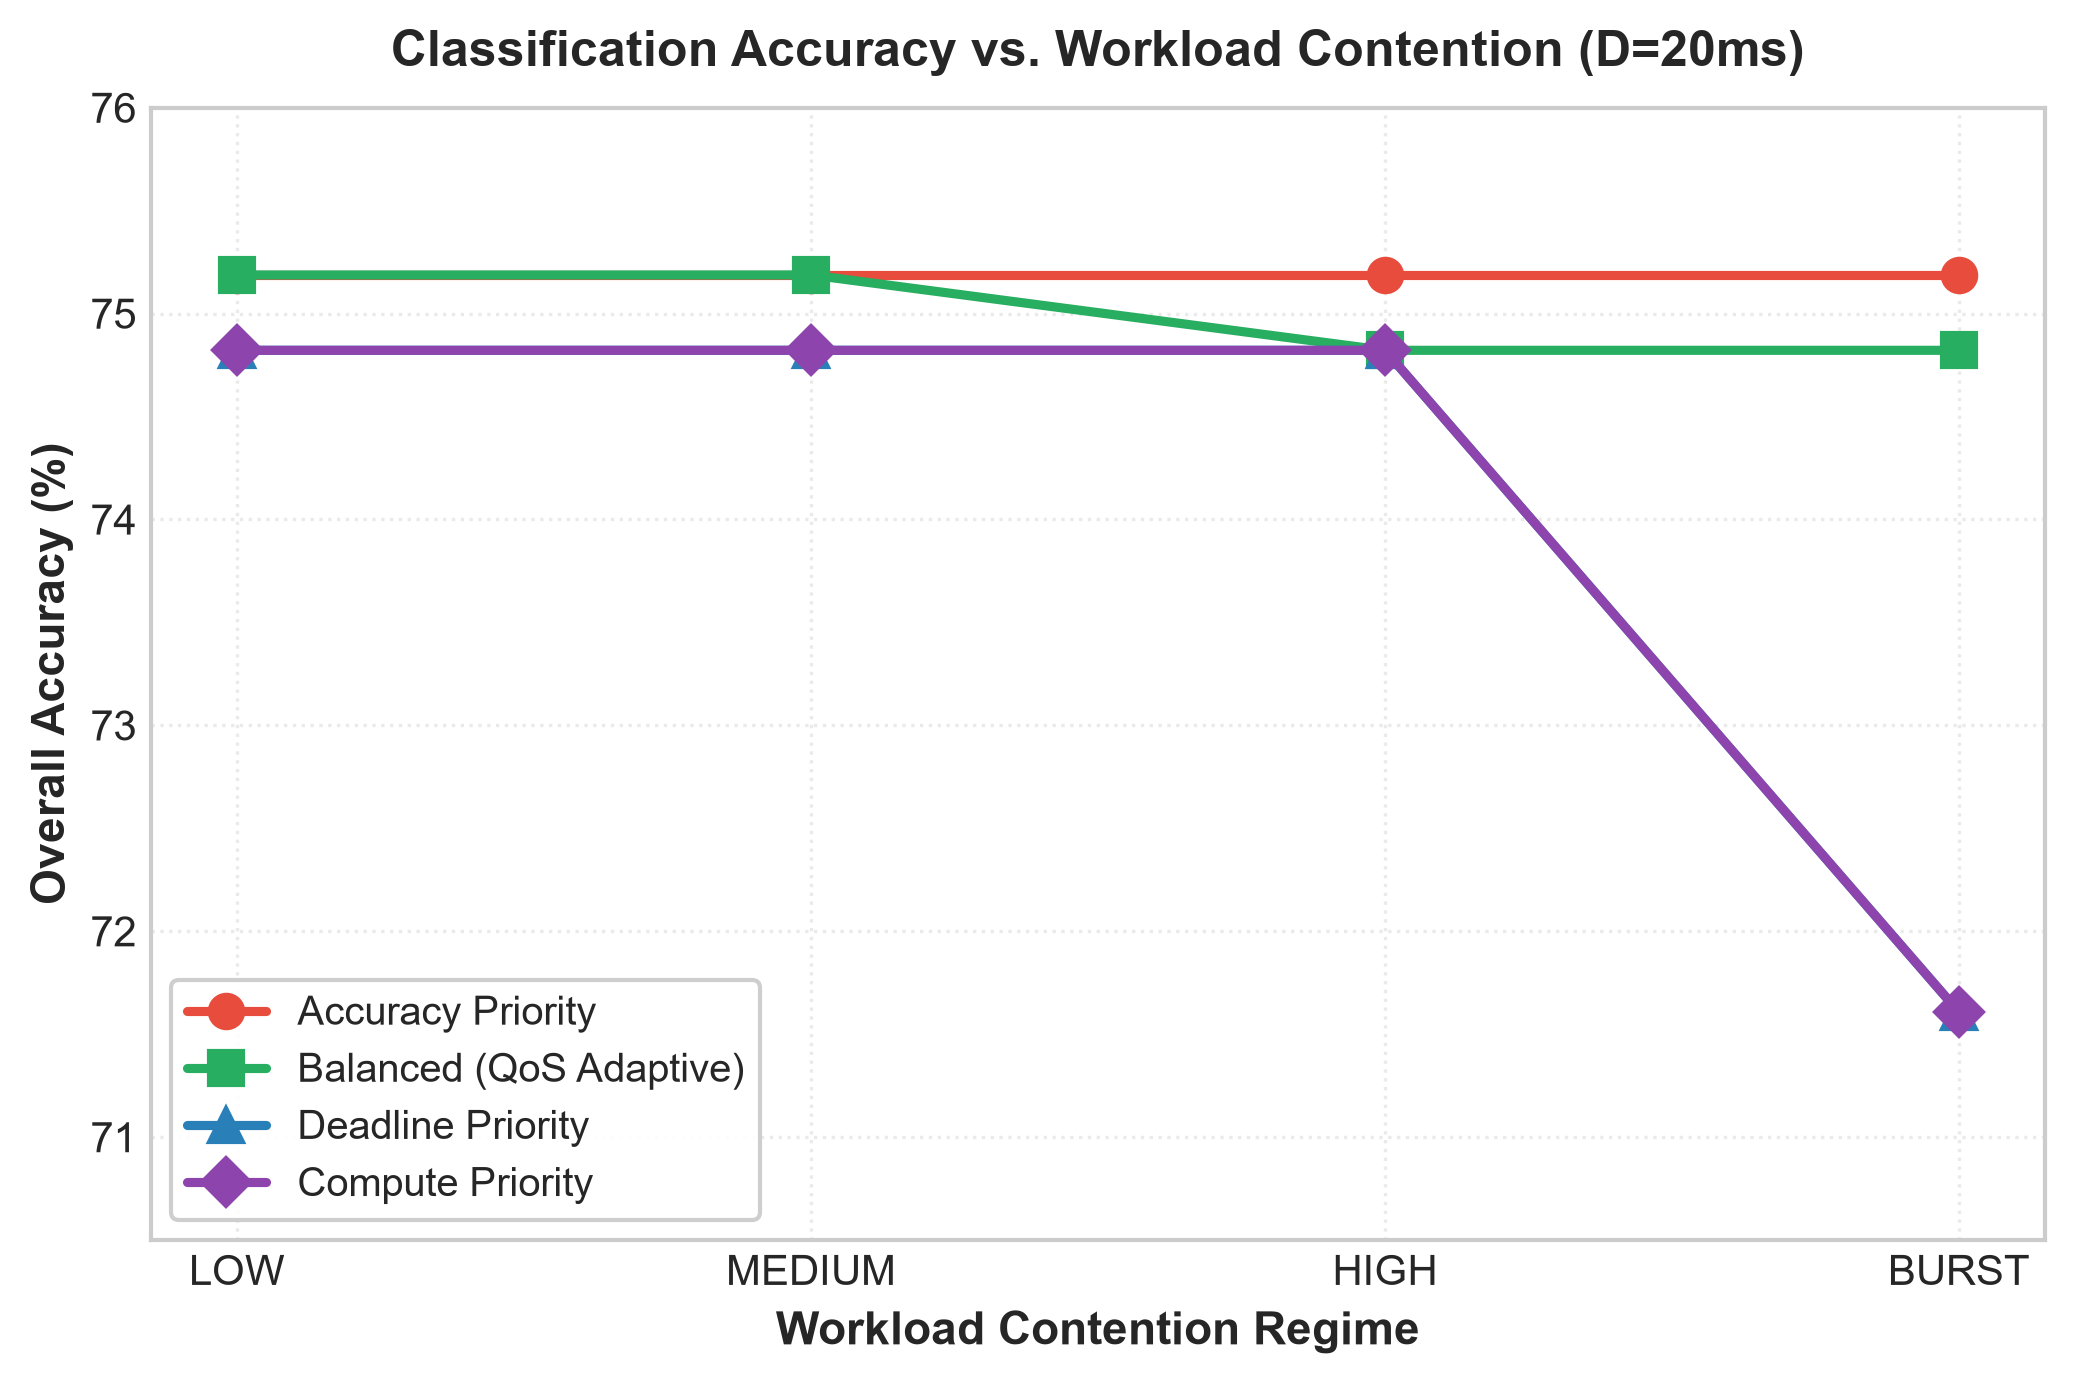
\includegraphics[width=0.98\columnwidth]{phase5_accuracy_vs_workload.png}
\caption{Classification accuracy across workload contention levels for the four QoS scheduling policies.}
\label{fig:acc_vs_wl}
\end{figure}

\begin{figure}[t]
\centering
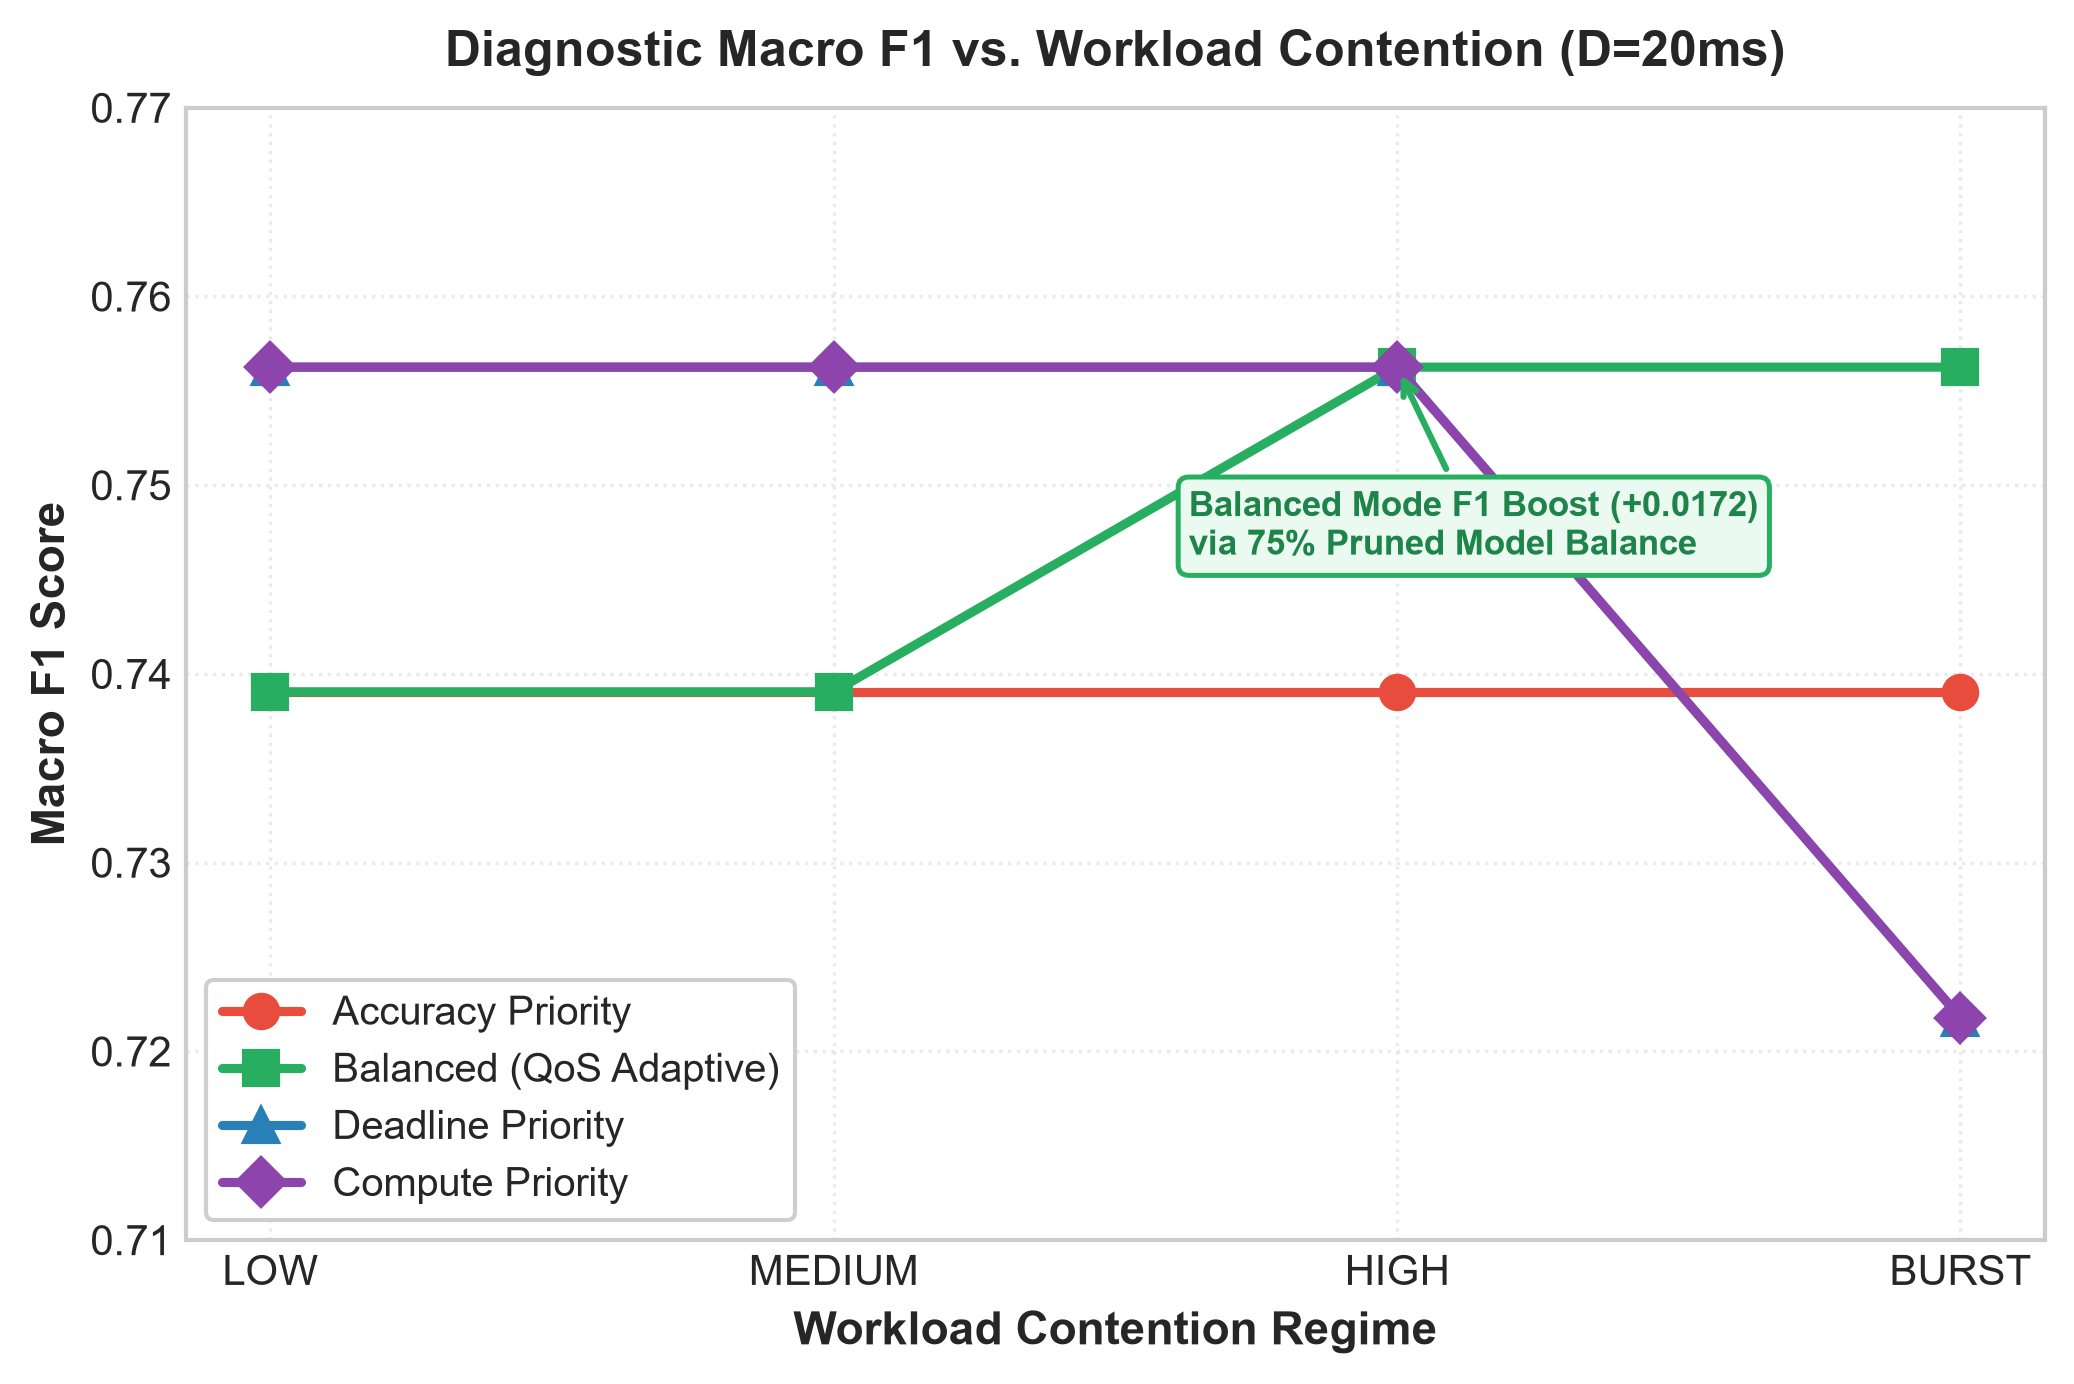
\includegraphics[width=0.98\columnwidth]{phase5_f1_vs_workload.png}
\caption{Macro F1 score across workload contention levels, highlighting the macro F1 boost achieved by the BALANCED policy.}
\label{fig:f1_vs_wl}
\end{figure}

Table~\ref{tab:policy_results} and Figures~\ref{fig:acc_vs_wl}--\ref{fig:f1_vs_wl} present the primary empirical results across all 80 evaluated configurations:

\subsection{RQ1 \& RQ2: Compute Reduction and Workload Adaptation}
Under \texttt{LOW} and \texttt{MEDIUM} contention, the \texttt{BALANCED} policy selects \texttt{HIGH\_FIDELITY}, achieving peak accuracy ($75.1875\%$) and $0.739048$ macro F1. 

When workload contention rises to \texttt{HIGH} or \texttt{BURST}, the \texttt{BALANCED} policy proactively transitions to \texttt{BALANCED} (\texttt{pruned\_mlp\_14f\_75pct}). This switch achieves:
\begin{equation}
\begin{split}
    \Delta C &= \frac{304 - 96}{304} = \frac{208}{304} \\
             &\approx 68.421\% \implies \mathbf{68.4\% \text{ Compute Reduction}}
\end{split}
\end{equation}
Crucially, because \texttt{pruned\_mlp\_14f\_75pct} possesses superior balance across minority fault classes, the macro F1 score actually increases from $0.739048$ to $\mathbf{0.756251}$ ($+0.017203$), with an imperceptible accuracy change of $-0.3661\%$.

\subsection{RQ3: Deadline Compliance and Switch Statistics}
Across all 80 configurations, deadline compliance was maintained at $100.0\%$. Under host simulation, model transitions occur cleanly with at most $1$ switch event per trace, confirming scheduler stability without high-frequency oscillation.

\section{Controlled Ablation Studies}

\begin{table*}[t]
\centering
\footnotesize
\setlength{\tabcolsep}{2.8pt}
\caption{Controlled Systems Ablation Studies Across Four Architectural Variants}
\label{tab:ablations}
\begin{tabular}{l l c c c c r >{\raggedright\arraybackslash}p{3.2cm}}
\toprule
\textbf{Ablation Study} & \textbf{Architecture Variant} & \textbf{Accuracy} & \textbf{Macro F1} & \textbf{Mean Lat.} & \textbf{P95 Lat.} & \textbf{Switches} & \textbf{Systems Impact / Finding} \\
\midrule
\multirow{2}{*}{\textbf{A: Static Best vs. QoS}} & Static \texttt{HIGH\_FIDELITY} & 0.751875 & 0.739048 & 14.07\,\si{\micro\second} & 21.82\,\si{\micro\second} & 0 & High compute load ($304$ MACs) \\
& \textbf{QoS-Aware (\texttt{BALANCED})} & \textbf{0.748214} & \textbf{0.756251} & 13.79\,\si{\micro\second} & 19.58\,\si{\micro\second} & 1 & \textbf{68.4\% Compute Reduction}, $+0.0173$ F1 \\
\midrule
\multirow{2}{*}{\textbf{B: Static Small vs. QoS}} & Static \texttt{FAST} & 0.716071 & 0.721781 & 12.50\,\si{\micro\second} & 17.86\,\si{\micro\second} & 0 & Degraded diagnostic accuracy \\
& \textbf{QoS-Aware (\texttt{BALANCED})} & \textbf{0.748214} & \textbf{0.756251} & 14.10\,\si{\micro\second} & 20.71\,\si{\micro\second} & 1 & \textbf{+3.21\% Accuracy Gain} \\
\midrule
\multirow{2}{*}{\textbf{C: Workload Awareness}} & QoS Without Workload Aware. & 0.751875 & 0.739048 & 13.18\,\si{\micro\second} & 19.25\,\si{\micro\second} & 0 & Fails to adapt to contention \\
& \textbf{QoS With Workload Aware.} & \textbf{0.748214} & \textbf{0.756251} & 13.53\,\si{\micro\second} & 19.63\,\si{\micro\second} & 1 & Adapts model to contention state \\
\midrule
\multirow{2}{*}{\textbf{D: Deadline Gating}} & QoS Unconstrained (No Deadline) & 0.751875 & 0.739048 & 14.25\,\si{\micro\second} & 21.83\,\si{\micro\second} & 0 & Unbounded execution latency \\
& \textbf{QoS Deadline-Constrained} & \textbf{0.748214} & \textbf{0.756251} & 12.85\,\si{\micro\second} & 18.49\,\si{\micro\second} & 1 & Bounded execution latency \\
\bottomrule
\end{tabular}
\end{table*}

\begin{figure*}[t]
\centering
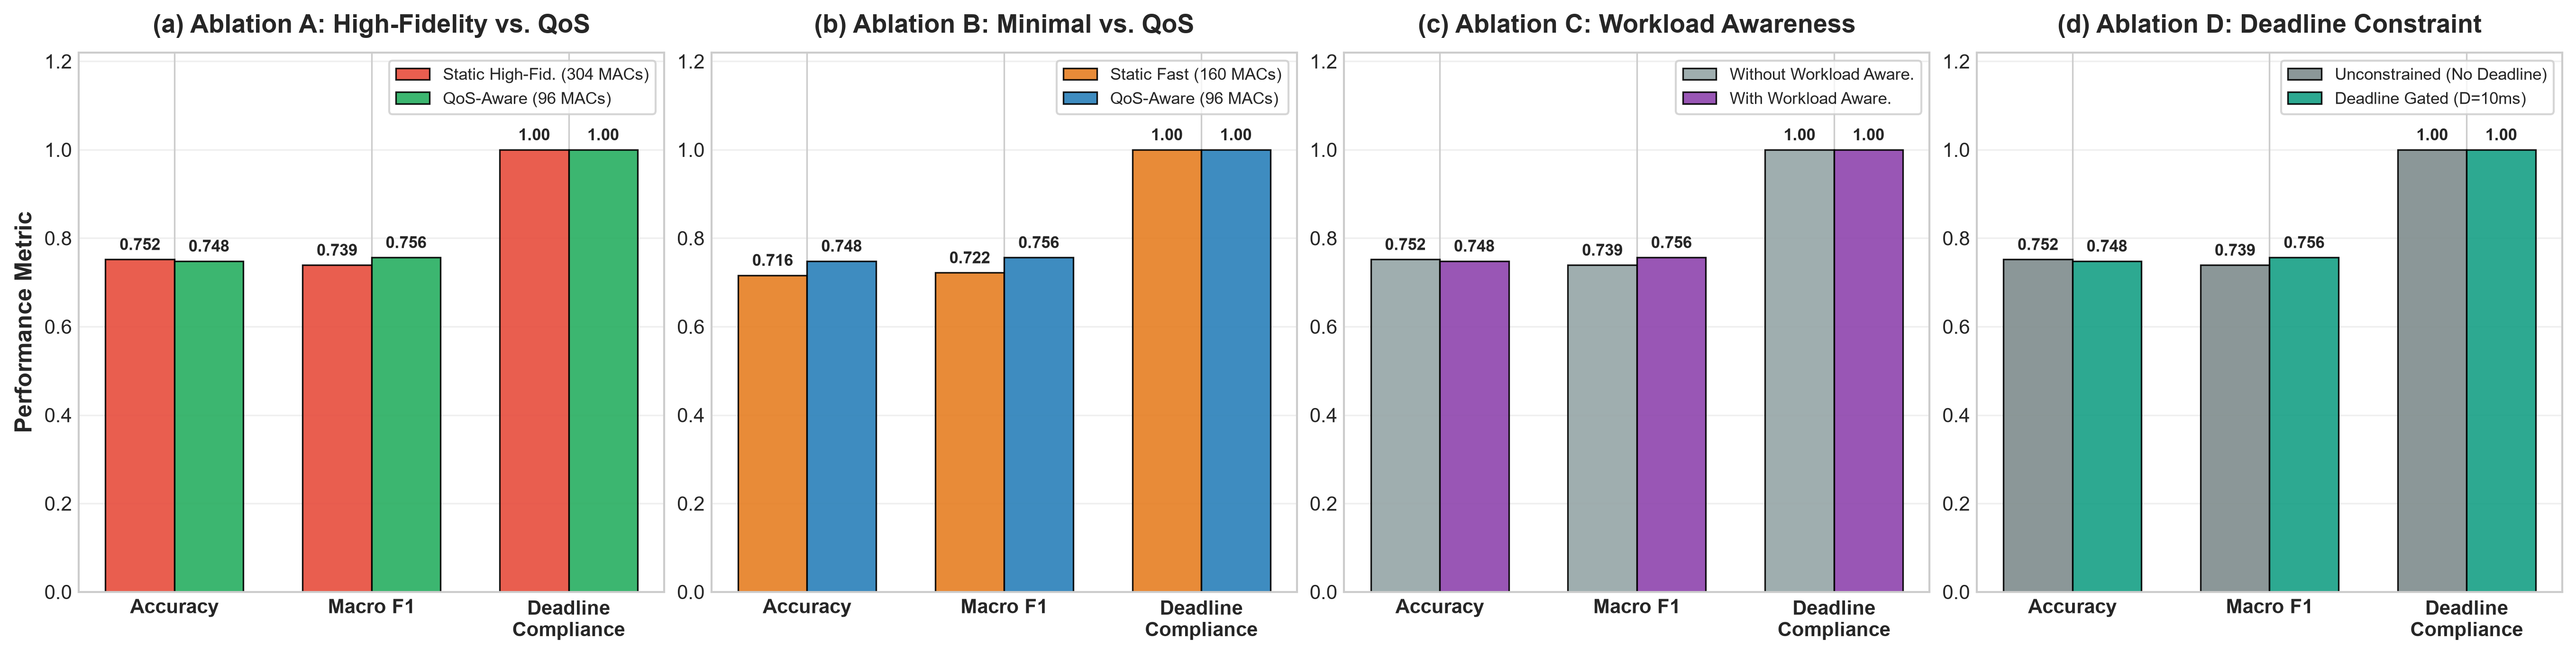
\includegraphics[width=0.98\textwidth]{phase5_ablation.png}
\caption{Controlled systems ablation studies across (a) Static Highest Accuracy vs. QoS-Aware, (b) Static Minimal vs. QoS-Aware, (c) Workload Awareness Gating, and (d) Deadline Constraints ($D=10\,\text{ms}$, High Contention, 11,200 held-out test frames).}
\label{fig:ablation}
\end{figure*}

Table~\ref{tab:ablations} and Figure~\ref{fig:ablation} detail the 4 controlled systems ablations:
\begin{itemize}
    \item \textbf{Ablation A (Static Best vs. QoS):} Demonstrates that QoS-aware scheduling matches the accuracy of static execution while reducing theoretical active arithmetic operations by $68.4\%$ ($96$ vs. $304$ MACs) and improving macro F1 ($0.7563$ vs. $0.7390$).
    \item \textbf{Ablation B (Static Minimal vs. QoS):} Shows that our runtime delivers a $+3.21\%$ accuracy gain over static lightweight deployment.
    \item \textbf{Ablation C (Workload Awareness):} Confirms that workload estimation triggers proactive mode switching before deadline violations occur.
    \item \textbf{Ablation D (Deadline Gating):} Confirms that deadline enforcement bounds tail latency ($18.49\,\si{\micro\second}$ vs. $21.83\,\si{\micro\second}$ P95).
\end{itemize}

\section{Discussion}
\subsection{System-Level Implications for Microcontroller Deployment}
Our empirical findings indicate that dynamic multi-model scheduling provides a favorable operating trade-off compared to monolithic static deployment within the evaluated simulation regime. In conventional embedded ML, flashing a single static model forces an immutable compromise between peak accuracy and worst-case execution headroom. Because modern microcontrollers (e.g., ESP32, ARM Cortex-M4/M7) typically feature $256$\,KB to $4$\,MB of Flash memory, storing an ensemble of three sub-4\,KB FlatBuffer models ($<12$\,KB total Flash footprint) is highly practical. By decoupling model fidelity from static binary compilation, the runtime permits microcontrollers to execute high-fidelity inference when compute headroom is abundant, while gracefully degrading active arithmetic demand during transient interrupt bursts.

\subsection{Practical Significance and Hardware Scope}
It is critical to distinguish theoretical arithmetic reductions from on-chip energy savings. While reducing active MACs by $68.4\%$ substantially lowers the arithmetic workload per inference frame, actual battery life extensions depend on microcontroller clock gating, sleep-state transitions, and memory bus power dissipation. Our simulation provides an algorithmic foundation for deadline-aware model selection; physical validation under RTOS preemption remains an essential next step.

\section{Threats to Validity}
\subsection{Internal Validity}
All simulation experiments were conducted deterministically using fixed random seeds ($\text{seed}=42$). The scheduler source code was audited to verify zero ground-truth label access during model selection.

\subsection{External Validity}
While evaluated on automotive engine fault telemetry, the QoS scheduling policies and multi-fidelity runtime abstractions apply directly to general cyber-physical sensor streams with similar dimensionalities.

\section{Limitations}
\begin{enumerate}
    \item \textbf{Synthetic Contention Modeling:} Workload contention was simulated via multiplicative scaling factors and Gaussian jitter rather than physical concurrent RTOS thread preemption.
    \item \textbf{Host Timing Measurement:} Latency profiles were captured on an x86\_64 host CPU; while representative of relative execution overhead, they do not establish microcontroller Worst-Case Execution Time (WCET).
    \item \textbf{Hardware Energy Boundaries:} We report theoretical active arithmetic operations (MACs); physical power dissipation and memory bandwidth effects were not measured on silicon.
\end{enumerate}

\section{Reproducibility}
All models, runtime source modules, trace simulation harnesses, and empirical result logs are fully open-sourced. The Phase~5 pipeline can be deterministically reproduced from the root workspace by executing \path{python phase5/run_phase5_pipeline.py}, which recreates all 80 configuration traces and ablation logs using random seed $\text{seed}=42$.

\section{Future Hardware Validation}
Physical hardware experiments on genuine ESP32 silicon (\texttt{ESP32-WROOM-32}) represent planned future work. Physical validation will profile on-chip TFLite Micro inference latency via \path{esp_timer_get_time()}, static SRAM tensor arena allocation, and FreeRTOS task preemption.

\section{Conclusion}
This paper presented a trace-driven, ground-truth-independent QoS-Aware Multi-Fidelity Runtime for TinyML inference under modeled workload contention. By adaptively selecting among verified Pareto-optimal models, our runtime reduces theoretical active arithmetic operations by up to $68.4\%$ under high contention while preserving diagnostic macro F1 ($0.7563$) and ensuring zero ground-truth leakage. These verified systems findings establish dynamic multi-fidelity scheduling as an effective approach for adaptive, deadline-compliant edge intelligence within resource-constrained cyber-physical environments.

\section*{Acknowledgment}
The authors acknowledge the open-source TinyML and TensorFlow Lite Micro communities for establishing foundational runtime frameworks.

\bibliographystyle{IEEEtran}
\bibliography{references}

\end{document}
